\documentclass{article}
\usepackage[final]{nips_2017}
\usepackage[utf8]{inputenc} % allow utf-8 input
\usepackage[T1]{fontenc}    % use 8-bit T1 fonts
\usepackage{hyperref}       % hyperlinks
\usepackage{url}            % simple URL typesetting
\usepackage{booktabs}       % professional-quality tables
\usepackage{amsfonts}       % blackboard math symbols
\usepackage{nicefrac}       % compact symbols for 1/2, etc.
\usepackage{microtype}      % microtypography
\usepackage{graphicx}
\usepackage[font=small, labelfont=bf]{caption}
\usepackage{subcaption}
\usepackage{float}
\usepackage{amsmath}
\title{Graph-Based Classification of Rock Climbing Difficulties}

\author{
  Rafael Hinojosa \\
  Microsoft Corporation \\
  Stanford University \\
  \texttt{rahinojo@stanford.edu} \\ 
  \And
  Cheng-Hao Tai \\
  Microsoft Corporation \\
  Stanford University \\
  \texttt{c2tai@stanford.edu} \\
  \And
  Aaron Wu \\
  Evisort Inc. \\
  - \\
  \texttt{aaron@evisort.com} \\
  %% examples of more authors
  %% \And
  %% Coauthor \\
  %% Affiliation \\
  %% Address \\
  %% \texttt{email} \\
  %% \AND
  %% Coauthor \\
  %% Affiliation \\
  %% Address \\
  %% \texttt{email} \\
  %% \And
  %% Coauthor \\
  %% Affiliation \\
  %% Address \\
  %% \texttt{email} \\
  %% \And
  %% Coauthor \\
  %% Affiliation \\
  %% Address \\
  %% \texttt{email} \\
}

\begin{document}
% \nipsfinalcopy is no longer used

\begin{center}

\includegraphics[width=3cm, height=0.7cm]{CS230}
\end{center}

\maketitle

\section{Introduction}	
At its inception, rock climbing was a fringe sport that grew out of a counter-culture scene in Yosemite Valley. In the decades since, climbing has evolved into a global sensation and is expected to prominently feature in the 2020 Olympic Games. Today, bustling rock climbing gyms can be found in nearly every American city with routes (a.k.a. problems) for every skill level from beginner to expert. To build skill and strength, climbers will typically create and follow training regimens of climbing problems at set difficulty levels, gradually progressing to problems of greater difficulty. Performing problem sets that are overly difficult runs a high risk of injury and frustration while an overly simple regimen results in suboptimal growth. Accurate grading of climbing routes, then, are integral to proper development of climbing expertise and the general enjoyment of the sport.

To address the need for accurate grading of climbing problems, we aim to create a classifier that assigns difficulty scores for climbing routes on an apparatus called the "Moonboard", shown in Figure 1. The Moonboard is a modular tool for setting and specifying various climbing routes. The base board is a fixed dimension that is constant for every Moonboard in existence. The configurations of holds on the board itself may change. Figure 1a depicts a configuration coined "Moonboard 2016". Given a specific Moonboard configuration, climbing problems can be set on them as shown in Figure 1b. In this way, climbers from around the world can participate in an online community where problems are created, practiced, and ranked. By creating a classifier that's capable of grading Moonboard routes, we will offer the climbing community a reliable alternative to the traditionally heuristically-based method of grading problems. Climbers will therefore be able to easily imagine new problems and receive a corresponding difficulty forecast. \textbf{Concretely, our classifier aims to take as input a set of holds on a Moonboard and predict an output difficulty label.}

\begin{figure}
\centering
\begin{subfigure}{.48\textwidth}
  \centering
  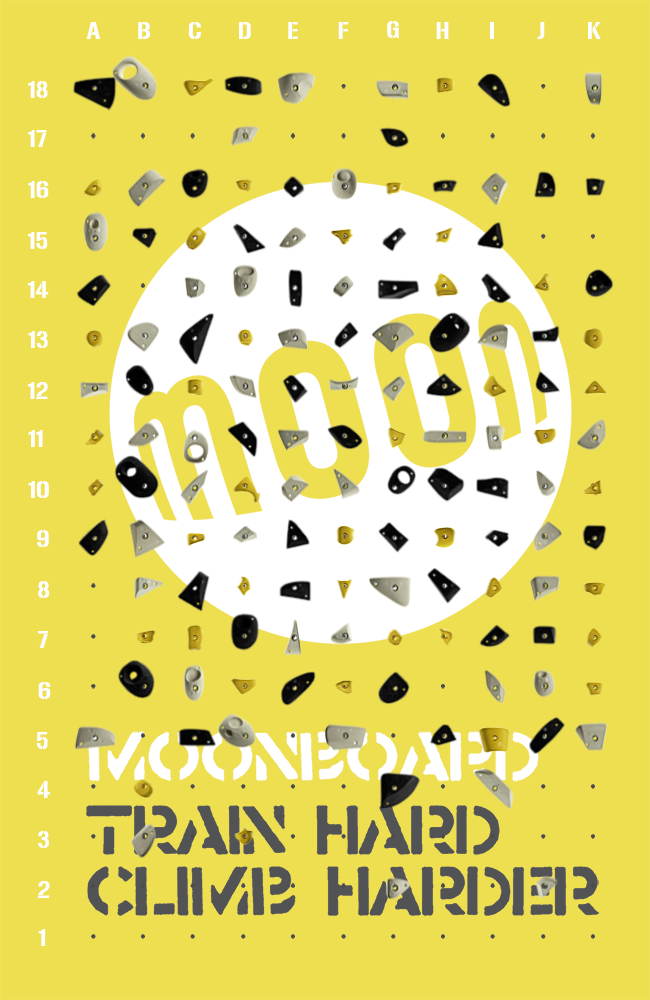
\includegraphics[width=.8\linewidth]{moonboard_stock}
  \caption{Moonboard 2016 configuration}
  \label{fig: Stock Moonboard}
\end{subfigure}
\begin{subfigure}{.48\textwidth}
  \centering
  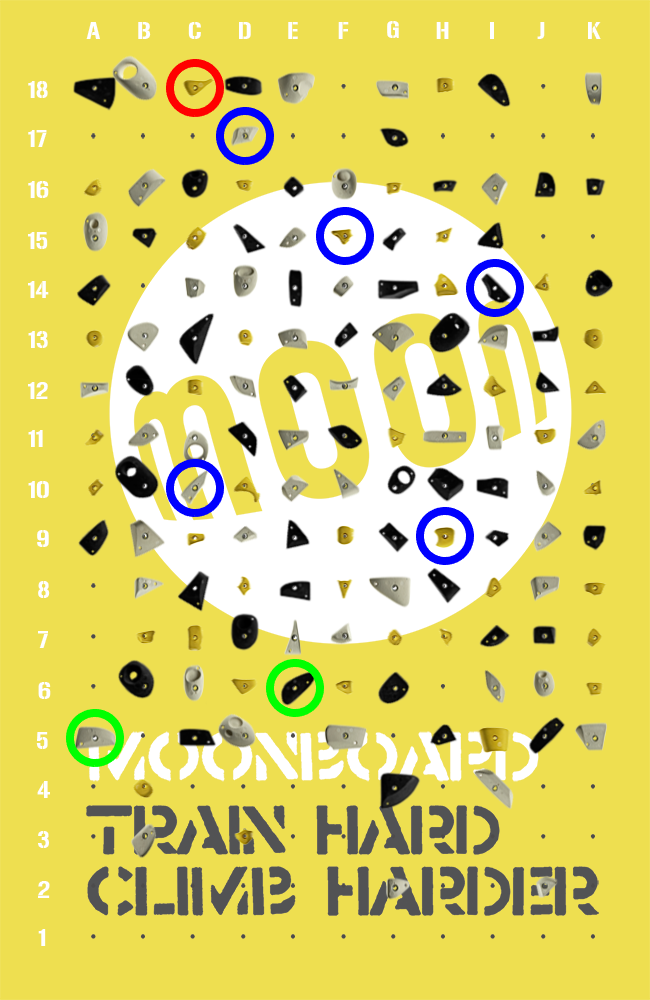
\includegraphics[width=.8\linewidth]{moonboard_1}
  \caption{A specific Moonboard problem}
  \label{fig: Moonboard Problem}
\end{subfigure}
\caption{Moonboard Training Apparatus}
\end{figure}

\section{Challenges}
The first challenge we face is data collection. Although Moonboard routes are readily available for the general public to \href{https://moonboard.com/}{view}, we anticipate having to mine the data from the Moonboard site. More details on the dataset will follow in Section 3. 

Once the data is available, we plan to model our classification problem using a graph structure and referencing [4] as a framework on which to build our model. In the paper presented in [4], a document classification problem was framed as a node classification task on a heterogenous graph (see Figure 2) composed of both words and documents. A 1:1 analogy can be applied for our problem wherein the document nodes are now problem nodes and words nodes are hold nodes. In this way, just as documents can be represented as a collection of nodes, Moonboard problems can be taken as a collection of holds. Defining the features for these graph nodes will be another challenge due to the heterogenous nature of the graph.

Finally, assuming that we can achieve satisfactory performance on our classification task, we wish to tackle either one of the two problems below:

\begin{enumerate}
\setlength\itemsep{0.1em}
\item Overcoming the inherent flaw of graph networks that require retraining of the entire network if a single new sample is introduced
\item Adding a generative component that can output a Moonboard problem, given an input difficulty (i.e. return a set of holds corresponding to a medium-level difficulty route)
\end{enumerate}

Task 1 is more aligned with a research-motivated direction while Task 2 (in combination with the base classifier that we will build), would have immense potential for a marketable product. 

\begin{figure}
\centering
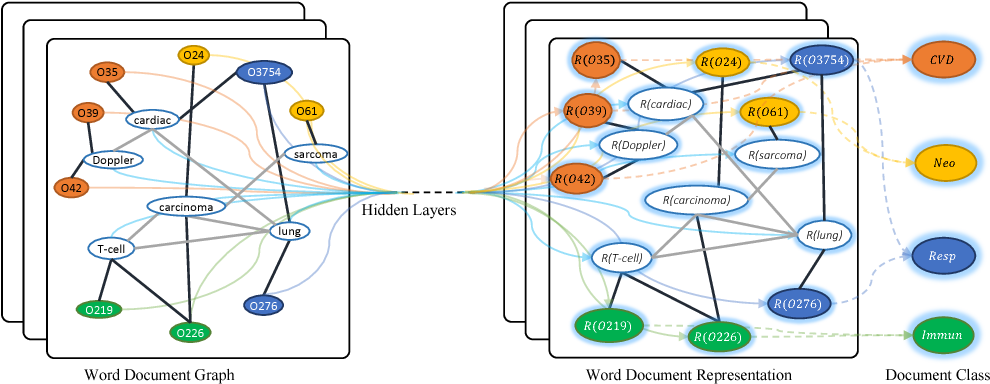
\includegraphics[width=.8\linewidth]{textGCN}
\caption{A heterogenous corpus graph for document classification using a Text Graph Convolutional Network. Nodes are both document entities and node entities. The different colors correspond to different node categories (notice only document nodes are colored). A direct analogy to Moonboard problems can be made by substituting documents for problems and words for nodes.}
\label{fig: Corpus graph for Text Graph Convolutional Network}
\end{figure}

\section{Dataset and Features}
As mentioned in Section 2, we plan on mining data directly from the Moonboard site. Our mined dataset will have the following schema:

\begin{itemize}
\setlength\itemsep{0.1em}
\item \texttt{Problem ID : int}
\item \texttt{Difficulty : int}
\item \texttt{Rating : int}
\item \texttt{Comments : string}
\item \texttt{Holds : list of tuples}
\end{itemize}

In total, we expect to mine a total of around 28,000 Moonboard problems for the Moonboard 2016 hold configuration. The \textbf{Holds} attribute is expected to be a list of tuples (row index, column index) of a particular hold in a Moonboard problem. These specific indexes are shown in Figure 1. Taken together, a set of hold tuples will define a specific Moonboard route (visually shown by the colored circles in Figure 1b).

\section{Preprocessing}
A significant task of our classifier will be to construct the graph representation of Moonboard problems. This task itself can be decomposed into two actions: 

\begin{itemize}
\setlength\itemsep{0.1em}
\item Setting node features
\item Defining edge weights on an adjacency matrix
\end{itemize}

For setting node features, we envision using some form of image encoding (i.e. transforming RGB images of Moonboard holds into 1D vectors) to create feature vectors for hold nodes. Under this paradigm, problem nodes could simply be a weighted or uniform average of corresponding hold vectors. It is also possible to create a bag-of-words inspired embedding of each hold and problem node by assigning each hold a one-hot vector (with the non-zero value corresponding to a predefined hold index) and having hold nodes be represented as a multi-hot vector where respective hold indexes are non-zero. 

As for defining edge weights, we plan on using a modified version of the adjacency relation defined in [4], shown below. The adjacency matrix self-loops are taken directly from the original definition but special attention will need to be placed in defining the distance relation amongst holds and the TFIDF calculation itself.

\[
    A_{ij}= 
\begin{cases}
    dist(i, j), & \text{if } i, j \text{ holds} \\
    \text{TFIDF}(j), & \text{if } i \text{ problem } j \text{ hold} \\
    1, & \text{if } i=j \\
    0, & \text{otherwise}
\end{cases}
\]

\section{Learning Method}
Our proposed learning method for the Moonboard problem classifier is [4]. On a related note, [3] offers a framework for simplifying the graph convolutional mechanism we are very interested in trying since [3]'s authors were able to improve upon the classification performance detailed in [4] by a nontrivial margin through a simpler model. 

To obtain our node-level features, we plan on building a preliminary image classifier using the residual unit idea proposed by [1]. Well-established network architectures such as Resnet-50 will be a good baseline model for us to begin exploration into this aspect of feature engineering. 

Lastly, we plan on exploring the usage of Conditional GANs outlined in [2] to assess whether a generative extension can be applied to our Moonboard classifier. Due to the nature of generative models, We expect that a generative component will require a reframing of our problem from a graph structure into a standard format. Intuitively, this requirement stems from the observation that a generative model applied to a graph dataset will simply aim to replicate that graph, which is not the behavior that we desire. 

\section{Evaluation}
For network evaluation, we plan on perform 80-20 splits on our mined data to create train-test datasets. On the training test itself, we will utilize hold-out subsets to monitor model training before running final validation on our test sets. Since we are currently framing our problem as a multi-class classification problem, we plan on applying the classical binary classification metrics (i.e. accuracy, precision, recall, F1 score) across the possible Moonboard difficulty categories. We expect that this approach of evaluating model performance on each difficulty class separately will enable us to easily identify class-specific issues.

Furthermore, given that our labels pertain to problem difficulties, it is also entirely possible to frame this as a regression problem. In this case, we would likely start by using regression-compatible metrics such as RMSE in conjunction with visualization tools like correlation plots to get a high-level intuition of our model performance. 

\section*{References}
\medskip
\small
[1] He, K., Zhang, X., Ren, S. \& Sun, J. \ Deep Residual Learning for Image Recognition \ {\it arXiv:1512.03385} \ (2015)

[2] Mirza, M. \& Osindero, S. \ Conditional Generative Adversarial Nets \ {\it arXiv:1411.1784} \ (2014)

[3] Wu, F., Zhang, T., de Souza Jr., A., Fifty, C., Yu, T., \& Weinberger, K. \ Simplifying Graph Convolutional Networks \ {\it Proceedings of the 36th International Conference on Machine Learning} \ (2019)

[4] Yao, L., Mao, C. \& Luo, Y. \ Graph Convolutional Networks for Text Classification \ {\it 33rd AAAI Conference on Artificial Intelligence (AAAI-19)}, 7370-7377 \ (2018)

\end{document}